\documentclass{article}


\usepackage[T2A]{fontenc}
\usepackage[utf8]{inputenc}
\usepackage[english,russian]{babel}
\usepackage[tbtags]{amsmath}
\usepackage{amsfonts,amssymb}

\hoffset -10mm
\voffset -7mm


\usepackage{mathrsfs}
\usepackage{graphicx}

\usepackage{float} % Иначе ругается на таблицу

\usepackage{amssymb,amsmath,amsthm,amsfonts}
\newtheorem{theorem}{Theorem}
\newtheorem{lemma}{Theorem}




\begin{document}
УДК 511.95 + 514.112

\begin{center}
	\textbf{
	Об отыскании множеств точек на плоскости с целочисленными расстояниями}
\end{center}


\footnotetext{Работа выполнена в Воронежском университете при поддержке РНФ, грант 16-11-101-25.}

Обозначим через $\mathbb{N}$ множество натуральных чисел, через $\mathbb{Z}$ --- множество целых чисел, через $\mathbb{R}$ --- множество действительных чисел, через $[x]$ --- наименьшее целое число, не превосходящее $x$, через $|A,B|$ --- расстояние между точками $A$ и $B$.
Для заданного $n\in \mathbb{N}, n\geq 3$ обозначим через $C_n$ множество таких последовательностей $M_1,M_2,...,M_n \in \mathbb{R}^2$, что $|M_i,M_j|\in\mathbb{N}$ для всех $1\leq i < j  \leq n$ и  $M_1,M_2,...,M_n$ не принадлежат никакой прямой.
Положим
$$
F(n)=\min\limits_{A\in C_n} d(A),
$$
где $d(A)$ --- диаметр $A$, т. е.
$$
d(A)=\max\limits_{x,y\in A}|x,y|
$$

В настоящей статье представлен алгоритм отыскания таких $A \in C_n$, что $d(A) = F(n)$.
Аналитические ограничения на $F(n)$ были получены в \cite{nashaStatya}:
для $n \geq 17$
	$$
		\max\left( \frac{n-5}{8}, 1 \right) \leq F(n) \leq \left( \frac{b (1+\log_2 n )\ln (1 + \log_2 n)}{e}\right)^{1+\log_2 n},
	$$
где $b$ --- константа из неравенств Чебышева.

? Дать здесь ссылку на неравенства Чебышева?




Рассмотрим сначала более общую задачу: для заданного $m \in \mathbb{N}$ отыщем (с точностью до движения) все такие множества $A \in C_n$, что $d(A) = m$.

Предположим, что такое множество найдено и его диаметр достигается на точках $P_1$ и $P_2$.
Введём на плоскости прямоугольную декартову систему координат так, что $P_1 = \left(-\frac{m}{2}; 0 \right)$, $P_2 = \left(\frac{m}{2}; 0\right)$.
Сведём задачу к конечному перебору, показав, что $A \subset P$, где $P$ --- конечное множество.
Действительно, пусть $P_{j} \in A$.
Тогда $|P_{j} P_1| \leq m$, $|P_{j} P_2| \leq m$, $|P_{j} P_1| \in \mathbb{Z}$ и $|P_{j} P_1| \in \mathbb{Z}$.
В качестве $P$ возьмём множество всех точек, удовлетворяющих вышеуказанному условию, т. е. множество точек пересечения пар всевозможных окружностей целого радиуса, не превосходящего $m$, с центрами в $P_1$ и $P_2$ соответственно.
Понятно, что $P$ содержит не более $2(m+1)^2$ точек; точное количество приведено ниже.

Координаты любой точки из $P$ могут быть выражены через радикалы:
$$
	P = \left\{
		\left(\left.  \frac{a^2-b^2}{2m} ; \pm\sqrt{a^2  - \left( \frac{a^2-b^2+m^2}{2m}\right)^2}  \right)	\right| 0 \leq a, b \leq m ; a+b \geq m
	\right\}
$$


Для оптимизации перебора сформируем три непересекающихся подмножества в множестве $P$:
$Q = \{P_j \in P | P_j = (x_j, 0)\}$;
$R = \{P_j \in P | P_j = (0, x_j), x_j \neq 0\}$;
$S = P \setminus \left( Q \cup R\right)$,
т. е. в множество $S$ попадают точки, у которых ни одна из координат не равна нулю.
Множества $Q$, $R$ и $S$ содержат $m+1$, $2\left\lbrack\frac{m+1}{2}\right\rbrack$ и $m^2$ точек соответственно.

Построим теперь граф $G$, вершины которого --- точки $P$;
вершины являются смежными, если расстояние между ними есть целое число, не превосходящее $m$.

На данном этапе задачу нельзя непосредственно свести к задаче о клике, решение которой описано, например, в \cite{BronKerbosh}:
клика может оказаться подмножеством множества $Q$, а значит, и оси абсцисс, что не удовлетворяет условию задачи (такую клику в дальнейшем будем называть тривиальной);
однако решение задачи о клике, описанное в \cite{BronKerbosh} --- алгоритм Брона-Кербоша --- может быть модифицирован таким образом, что не найдёт тривиальные клики.
Для этого достаточно на начальном этапе каждой ветви перебора не использовать вершины, принадлежащие $Q$, как клики мощности 1.
При такой модификации алгоритма его сложность, очевидно, не увеличивается и, как доказано в работе \cite{Tomita}, не превосходит $O(3^{m^2/3})$.


Автором найден способ оптимизировать дальнейший перебор с учётом того, что рёбер в изучаемом графе достаточно мало.
Будем исключать вершины $P_j$ из графа по следующим правилам до тех пор, пока это возможно:

а) Если $P_j \in Q$ и $P_j$ не соединена ребром ни с какой точкой из $S \cup R$, то $P_j$ можно исключить, и вместе с ней можно исключить точку, симметричную $P_j$ относительно начала координат.

б) Если $P_j \in P$ и $P_j$ имеет менее $n-1$ смежных вершин, то $P_j$ можно исключить вместе с одной (в случае, когда $P_j \in Q \cup R$) или даже тремя (в случае, когда $P_j \in S$) точками, симметричными $P_j$ относительно осей координат.

Использование симметрии позволяет не проводить подсчёт смежных вершин для некоторых точек, что немаловажно для ускорения работы алгоритма на ЭВМ.
Заметим, что при реализации алгоритма симметричные точки целесообразно хранить парами или группами по 4.

Сложность каждой проверки правила (а) для множества $Q$ не превосходит $O(m^3)$, правила (б) для всего множества $P$ --- $O(m^4)$.

Для примера: однократное применение правила (б) к каждой точке из множества $Q$ для $m=413$ и $n=29$ заняло на используемой ЭВМ менее семи минут и привело к уменьшению количества вершин графа с 171396 до 2084.

? Может быть, нужно провести расчёты для одной и той же пары с применением оптимизаций и без него?

После того, как дальнейшее сокращение графа $G_k$, полученного из графа $G$ применением этих правил $k$ раз, станет невозможным, начнём применять следующее рекуррентное правило, фактически обобщающее правила (а) и (б):

в)
Для каждой вершины $P_j$ через $\varphi(P_j,G_k)$ обозначим подграф графа $G_k$, состоящий из вершины $P_j$ и всех вершин, смежных с ней.
Если в графе $\varphi(P_j,G_k)$ отсутствует нетривиальная клика мощности $n$ (это определяется с помощью модифицированного алгоритма Брона-Кербоша), то вершину $P_j$ и вершины, симметричные ей относительно осей координат, можно исключить.

Если же нетривиальная клика найдена, то задача решена.

Целесообразно начать применение этого правила с вершины, имеющей минимальное числ смежных вершин.

Очевидно, что рекурсия конечна.
Она заканчивается в одном из следующих случаев:

1) мощность графа $G_k$, полученного на $k$-й итерации, меньше $n$;

2) граф $G_k \subset Q$;

3) нетривиальная клика найдена.



Отыщем теперь с помощью приведённого алгоритма $F(n)$ для произвольного $n \in \mathbb{N}$.

Очевидно, что $F(3) = 1$.
Положим $m_1=1$, $n_1=3$.
На $k$-м шаге будем искать $A \in C_{n_k}$, такое, что $d(A) = m_k$.
Если такое множество найдено, это означает, что $F(n_k)=m_k$,
в таком случае увеличим количество точек, т. е. положим $n_{k+1} = n_k +1$, $m_{k+1} = m_k$;
в противном случае увеличим диаметр, т. е. $n_{k+1} = n_k$, $m_{k+1} = m_k +1$.



Автору удалось создать программу для ЭВМ и провести расчёты для множеств, диаметр которых не превышает 986.
Результаты вычислений представлены в таблице 1.


\begin{table}[H]
\caption{Значения $F(n)$}
\label{tabular:pc_counted}
\begin{center}
\begin{tabular}{|c|c|c|c|c|c|c|c|c|c|c|c|}
\hline
\textbf{n}    &  3 & 4 & 5 & 6 &  7 &  8 &  9 & 10 & 11 & 12 & 13 \\
\hline
\textbf{F(n)} &  1 & 4 & 7 & 8 & 17 & 21 & 29 & 40 & 51 & 63 & 74  \\
\hline
\hline
\textbf{n}    &  14 &  15 &  16 &  17 &  18 &  19 &  20 &  21 &  22 &  23 &  24 \\
\hline
\textbf{F(n)} &  91 & 104 & 121 & 134 & 153 & 164 & 196 & 212 & 228 & 244 & 272  \\
\hline
\hline
\textbf{n}    &  25 &  26 &  27 &  28 &  29 &  30 &  31 &  32 &  33 &  34 &  35 \\
\hline
\textbf{F(n)} & 288 & 319 & 332 & 364 & 396 & 437 & 464 & 494 & 524 & 553 & 578  \\
\hline
\end{tabular}
\begin{tabular}{|c|c|c|c|c|c|c|c|c|c|c|}
\hline
\textbf{n}    &  36 &  37 &  38 &  39 &  40 &  41 &  42 &  43 &  44 & 45\\
\hline
\textbf{F(n)} & 608 & 642 & 667 & 692 & 754 & 816 & 897 & 959 & 986 & $986<F(45)\leq 1038$\\
\hline
\end{tabular}
\end{center}
\end{table}


Исходный код программы для ЭВМ, с помощью которой производились расчёты, размещён по адресам (гитхаб) и (сайт матфака) на условиях лицензии GNU GPLv3. 


При проведении расчётов на ЭВМ, поддерживающих параллельные вычисления (например, лабораторных ЭВМ, имеющих многоядерный процессор) наиболее целесообразным представляется поиск систем с большим диаметром <<заранее>>.

Пусть имеется возможность исполнять $q$ параллельных процессов.
Всякий раз, когда количество выполняющихся процессов меньше максимально допустимого (т. е. после того, как предыдущий процесс завершил свою работу, либо перед началом вычислений), определим мощность и диаметр множества, которое будет искать запускаемый процесс, применяя следующие три правила до тех пор, пока это возможно:

(i)
Изначально положим $m_1=1$, $n_1=3$.

(ii)
Если множество с диаметром $m_k$ мощности $n_k$ было найдено ранее, положим $n_{k+1} = n_k +1$, $m_{k+1} = m_k$.

(iii)
Если ранее было установлено, что искомого множества с диаметром $m_k$ мощности, не превосходящей $n_k$, не существует,
или если в данный момент выполняется процесс, отыскивающий такое множество, положим $n_{k+1} = n_k$, $m_{k+1} = m_k+1$.

Как только достигнуто такое $k$, что данные правила применить нельзя, следует запустить процесс, отыскивающий множество с диаметром $m_k$ мощности $n_k$.


С ростом диаметра множества время поиска увеличивается очень значительно.
Например, отыскание оптимального мноества из 4 точек занимает менее 0.1 секунды на рабочей ЭВМ автора;
проверка наличия множества мощности 14 с диаметром 91 --- около 0.5 секунды;
вычисление же $F(44)$ при известной $F(43)$ потребовало нескольких суток работы кластера из 30 лабораторных ЭВМ.



Приведём наиболее примечательные, на взгляд автора, примеры найденных множеств.

Так, для $n=4$ имеем:
$$
\left\{\left( -2 ; 0\right),\left( 2 ; 0\right),\left( \frac{3}{2} ; \frac{\sqrt{15}}{2}\right),\left( 1 ; 0\right)\right\}
$$

$$
\left\{\left( -2 ; 0\right),\left( 2 ; 0\right),\left( \frac{3}{2} ; \frac{\sqrt{15}}{2}\right),\left( -\frac{3}{2} ; \frac{\sqrt{15}}{2}\right)\right\}
$$


\begin{figure}[h]
\center{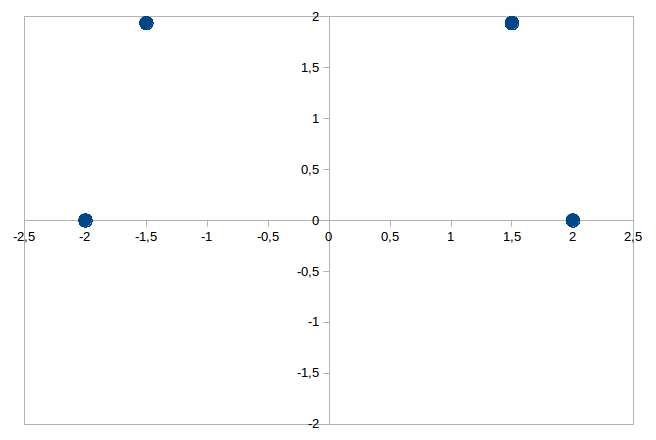
\includegraphics[width=0.45\linewidth]{illustr/sct-4-4_1.png}}
\caption{$n=4$, первый случай}
\label{ris:image}
\end{figure}

\begin{figure}[h]
\center{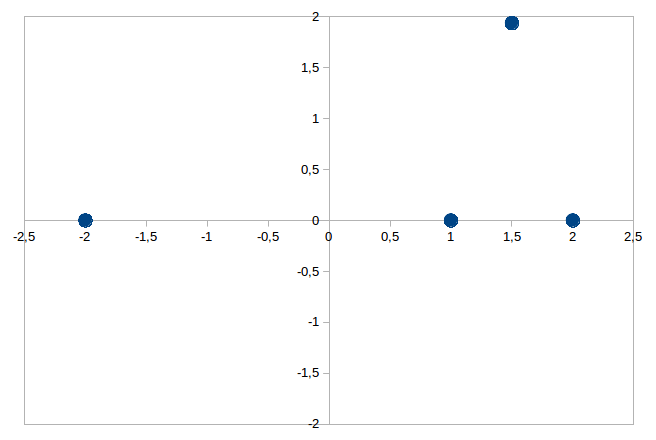
\includegraphics[width=0.45\linewidth]{illustr/sct-4-4_2.png}}
\caption{$n=4$, второй случай}
\label{ris:image}
\end{figure}

Для $n=5$ оптимальное расположение единственно с точностью до движения:
$$
\left\{\left( -\frac{7}{2} ; 0\right),\left( \frac{7}{2} ; 0\right),\left( 0 ; \frac{\sqrt{15}}{2}\right),\left( \frac{1}{2} ; 0\right),\left( -\frac{1}{2} ; 0\right)\right\}
$$


\begin{figure}[h]
\center{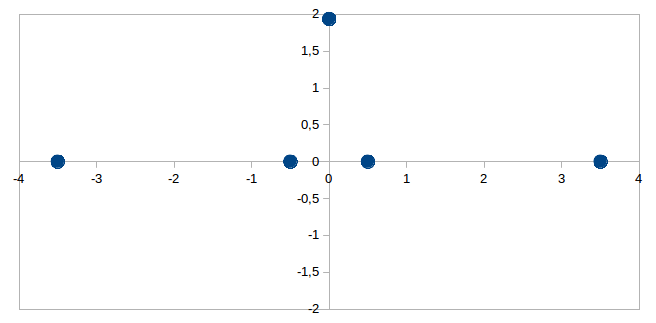
\includegraphics[width=0.45\linewidth]{illustr/sct-5-7.png}}
\caption{$n=5$}
\label{ris:image}
\end{figure}



Автор выражает благодарность проф. Е. М. Семёнову за ценные советы и плодотворное обсуждение.


%%%%%%%%%%%%%%%%%%%%%%%%%%%%%%%%%


\newpage

\addcontentsline{toc}{chapter}{\bibname}
\begin{thebibliography}{99}

\bibitem{nashaStatya} Авдеев Н. Н., Семёнов Е. М. О множествах точек на плоскости с целочисленными расстояниями. --- в печати.

\bibitem{BronKerbosh} Bron C., Kerbosh J. (1973), Algorithm 457 — Finding all cliques of an undirected graph, Comm. of ACM, 16, p. 575—577.

\bibitem{Tomita} Etsuji Tomita, Akira Tanaka, Haruhisa Takahashi (2006), The worst-case time complexity for generating all maximal cliques and computational experiments, Theoretical Computer Science, Vol 363, Issue 1, ISSN:0304-3975, p. 28-42.

\end{thebibliography}









%Замечание
%\begin{remark} Отметим, что доказательство теоремы \ref{theo1} 
%может быть распространено на случай ...
%\end{remark}

%Определение
%\begin{definit} Будем называть ...
%\end{definit}

%Предложение
%\begin{propos} Пусть выполняются следующие неравенства...
%\end{propos}

%\begin{figure}[ht]
%\centering
%\includegraphics{1kriv80}
%\caption{Многообразие точек смены кратности.}
%\end{figure}


%===============Список литературы==================



\end{document}
